\documentclass{beamer}
\usetheme{Madrid}
\usecolortheme{default}


\usepackage[T1]{fontenc}
\usepackage[utf8]{inputenc}
\usepackage{amsmath,amssymb,bm,mathtools}
\usepackage{xcolor}
\usepackage{hyperref}
\usepackage{microtype}

\graphicspath{{./figures/}}
\usepackage{booktabs}


\title[Project 2]{Project 2}
\subtitle{CS 332, Fall 2025}
\author{Ben Cole \and Koshi Harashima}
\date{22 October, 2025}

\begin{document}

\maketitle

\begin{frame}{Outline}
  \tableofcontents
\end{frame}

\section{Part1}


\subsection{A}
\begin{frame}{Part:A - Adversarial Fair Playoffs}
\textbf{Model}
\begin{itemize}
  \item Each round: draw \(x \sim \mathrm{Uniform}[0,1]\).
  \item Assign \(x\) to the action with smallest cumulative payoff so far; others get 0.
\end{itemize}
\textbf{Algorithms / learning rates}
\begin{itemize}
  \item No learning: \(\epsilon = 0\) (uniform random).
  \item Theoretical: \(\epsilon = \sqrt{\ln k / n}\).
  \item FTL: follow the current leader (or very large \(\epsilon\)).
\end{itemize}
\textbf{Setup}: e.g., \(k=10\), \(n=1000\), 50 trials (Monte Carlo).
\end{frame}

\begin{frame}{Part:A - Results}
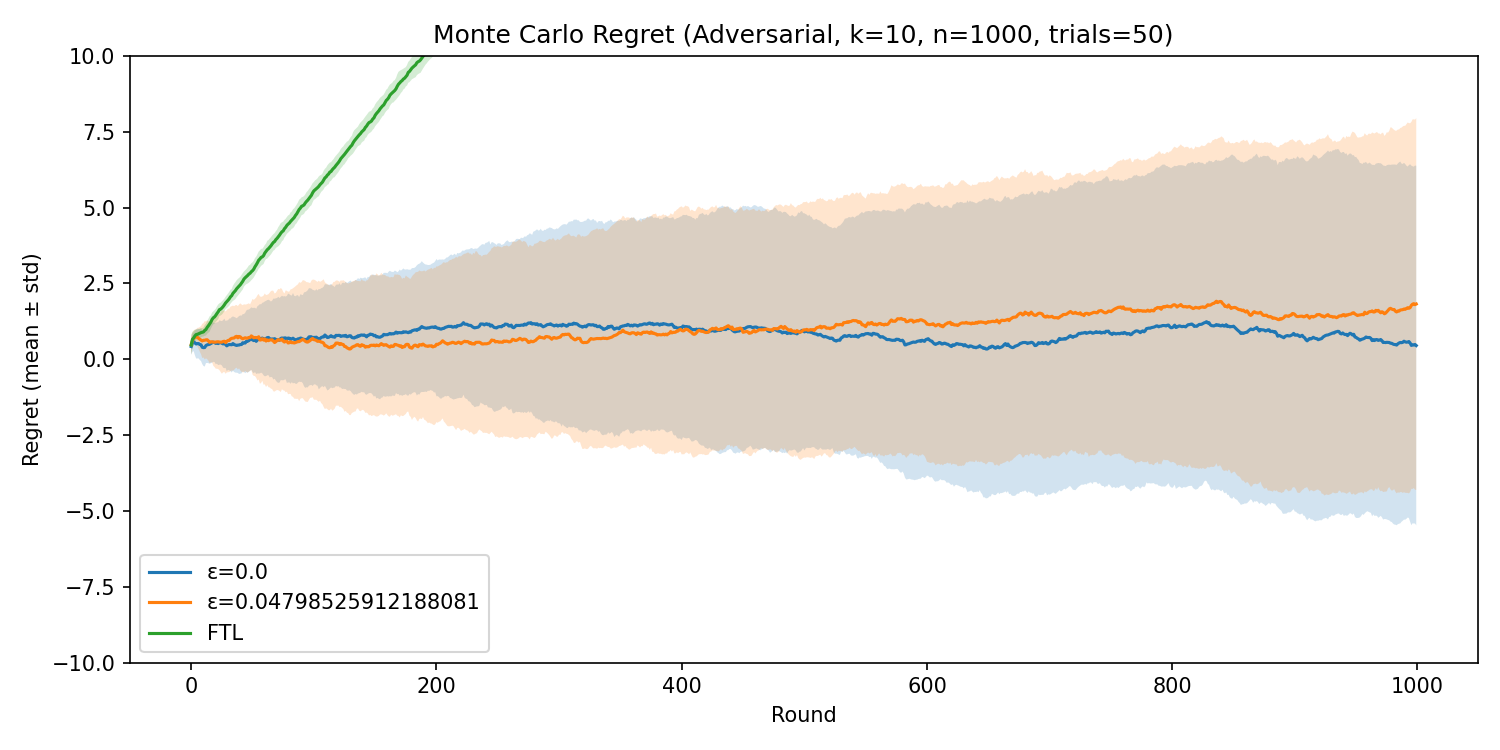
\includegraphics[width=0.9\textwidth]{figures/adv_mc_regret.png}

\end{frame}

\subsection{B}


\subsection{C}
\begin{frame}{Part:C}
In this part, we collect data from Japanese Pachinko (slot machine in Japan).\\
Here's our setting. Simple model with state transition model.
\begin{itemize}
    \item There are two conditions(unobservable)
    \begin{itemize}
        \item Normal condition
        \item Rush condition
    \end{itemize}
    \item In each setting, the chance of winning or losing is assigned.
\end{itemize}
\begin{itemize}
    \item we collect folloing data; 
    \begin{itemize}
        \item 1. payoff
        \item 2. probability of winning for each state.
        \item 3. probability of condition transition for each state.
    \end{itemize}
    \item there's five famous machines whose payoffs and probabilities differ from each other.
\end{itemize}
\end{frame}

\begin{frame}{C. Description of Machines}
5 machines; Tokyo Gouhl, Gundam Unicorn, Madoka Magica, Evangelion, Re.ZERO.
\begin{itemize}
    \item 1. Tokyo Gouhl
    \begin{itemize}
        \item low probability of winning, highest profit
    \end{itemize}
    \item 2. Gundam Unicorn
    \begin{itemize}
        \item middle
    \end{itemize}
    \item 3. Madoka Magica 
    \begin{itemize}
        \item middle
    \end{itemize}
    \item 4. Evangelion
    \begin{itemize}
        \item In rush state, profit is insane.
    \end{itemize}
    \item 5. Re.ZERO
    \begin{itemize}
        \item high average performance
    \end{itemize}
\end{itemize}
\end{frame}

\begin{frame}{Appendix: Image}
    
\end{frame}
\begin{frame}{C. Result}

    
\end{frame}
\begin{frame}{C. Graghs}

    
\end{frame}


    

\subsection{D}


\section{Usage of AI}
\begin{frame}{Usage of AI}
    AI was used for coding; final review and responsibility by the authors.
\end{frame}

\end{document}